\begin{frame}
    \titlepage
\end{frame}

\tikzset{
    stackBox/.style={very thick},
    allocBox/.style={dashed,very thick,fill=blue!20},
    onStack/.style={thick},
    frameOne/.style={fill=blue!15},
    frameTwo/.style={fill=red!15},
    markLine/.style={blue!50!black},
    markLineB/.style={red!90!black},
    hiLine/.style={red!90!black},
}

\begin{frame}{logistics: ROP assignment}
\end{frame}

\section{Memory Safety Research Overview}

\begin{frame}{2013 memory safety landscape}
    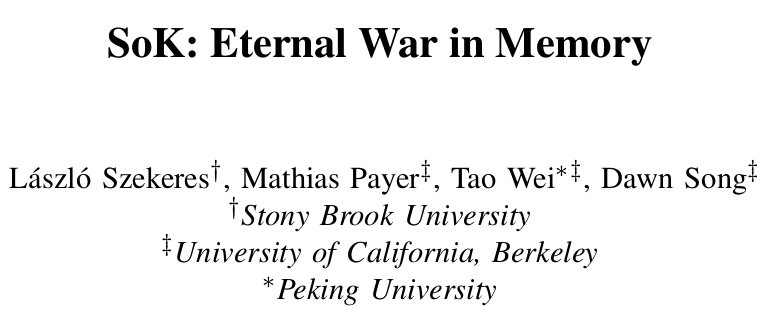
\includegraphics[width=1.0\textwidth]{SoK-eternal-title}
\end{frame}

\begin{frame}{2013 memory safety landscape}
    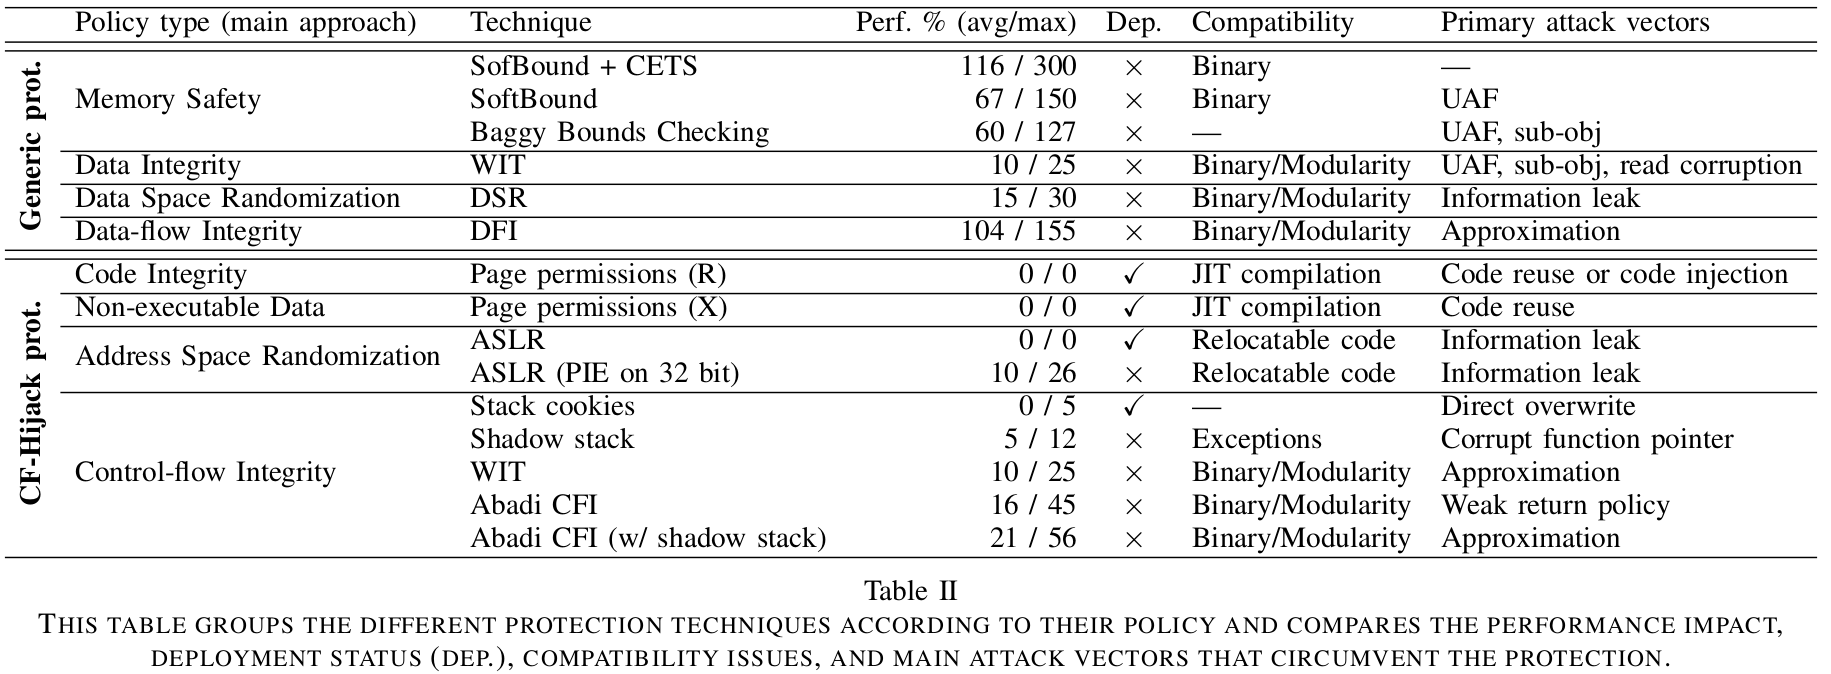
\includegraphics[width=1.05\textwidth]{SoK-table}
\end{frame}

\begin{frame}{different design points}
    \begin{itemize}
    \item memory safety most extreme --- disallow out of bounds
        \begin{itemize}
        \item usually even making out-of-bounds pointers
        \end{itemize}
    \item relaxations:
        \vspace{.5cm}
    \item separate `safe' data like buffers and `unsafe' data like return addresses
        \begin{itemize}
        \item instead of all objects from each other
        \end{itemize}
    \item check only writes or only reads
    \item \ldots
    \end{itemize}
\end{frame}


\begin{frame}{the mitigations}
    \begin{itemize}
        \item things the OS/compiler can do
        \item assume software won't or can't be fixed
        \item goal: make programs better despite lack of effort by developers
        \item in practice: hard to get >10\% overhead mitigations deployed
        \vspace{.5cm}
    \item what else can we do?
    \end{itemize}
\end{frame}

\begin{frame}<1-2>[fragile,label=altTechs]{alternative techniques}
    \begin{itemize}
        \item \myemph<2>{memory error detectors} --- to help with software \textbf{testing}
            \begin{itemize}
            \item reliably detect single-byte overwrites, use-after-free
            \item bitmap for every bit of memory --- should this be accessed
            \item \textbf{not} suitable for stopping exploits
            \item examples: AddressSanitizer, Valgrind MemCheck
            \end{itemize}
        \item \myemph<3>{automatic testing tools} --- run programs to trigger memory bugs
        \item \myemph<4>{static analysis} --- analyze programs and either
            \begin{itemize}
            \item find likely memory bugs, or
            \item prove absence of memory bugs
            \end{itemize}
        \item \myemph<5>{better programming languages}
    \end{itemize}
\end{frame}

\section{Debugging memory error detectors}

\begin{frame}{recall: baggy bounds}
    \begin{itemize}
    \item check on \myemph{pointer manipulation}
    \item make sure pointer maps to same object
        \vspace{.5cm}
        \item more typical solution: check on \myemph{read/write}
        \item goal was to run programs safely --- can also \myemph{find bounds errors}
    \end{itemize}
\end{frame}

\begin{frame}{testing workflow}
    \begin{itemize}
    \item use a tool like baggy bounds to make errors \textbf{crash}
    \item run \myemph{thorough} tests of software; fix any crashes
        \vspace{.5cm}
    \item idea: overhead is okay when debugging
    \end{itemize}
\end{frame}

\begin{frame}{can you use Baggy Bounds?}
    \begin{itemize}
    \item not released in useable form as far as I know
    \item but there are alternative tools that are available
    \item \ldots which are better fits for testing
    \end{itemize}
\end{frame}

\begin{frame}{AddressSanitizer}
    \begin{itemize}
    \item like baggy bounds:
        \begin{itemize}
        \item big lookup table
        \item lookup table set by memory allocations
        \item compiler modification: change stack allocations
        \end{itemize}
    \item unlike baggy bounds:
        \begin{itemize}
        \item check reads/writes (instead of pointer computations)
        \item only detect errors that read/write \myemph{between objects}
        \item object sizes not padded to power of two
        \item table has info for every single byte (more precise)
        \end{itemize}
    \end{itemize}
\end{frame}

\begin{frame}[fragile,label=asanVBounds]{adding bounds-checking example}
\lstset{
    language=C++,
    style=small,
    moredelim={**[is][\btHL<2>]{~2~}{~end~}},
}
\begin{lstlisting}
void vulnerable(long value, int offset) {
    long array[10] = {1,2,3,4,5,6,7,8,9,10};
    // generated code: (added by AddressSanitizer)
    ~2~if (!lookup_table[&array[offset]] == VALID) FAIL();~end~
    array[offset] = value;
    do_something_with(array);
}
\end{lstlisting}
    \begin{itemize}
        \item AddressSanitizer: crashes only if \lstinline|array[offset]| isn't part of any object
            \begin{itemize}
            \item but no extra space --- single-byte precision
            \end{itemize}
    \end{itemize}
\end{frame}

\begin{frame}[fragile,label=asanStackLayout]{AddressSanitizer stack layout}
    \begin{tikzpicture}
        \begin{scope}[x=1.7cm]
    \draw[stackBox] (0, 0) rectangle (5, -6);
            \draw[onStack] (0, 0) rectangle (5, -.5)
        node[midway] (arrayLoc) { return address (for \texttt{vulernable()}) };
    \begin{visibleenv}<2>
        \node[anchor=west] at (5.25, -.25) { $\approx$ \tt array[0x13]};
        \node[anchor=west] at (5.25, -3.75) { $\approx$ \tt array[0xa]};
    \end{visibleenv}
    \draw[onStack] (0, -.5) rectangle (5, -1)
        node[midway] { saved \tt\%rbp };
    \draw[onStack] (0, -1) rectangle (5, -1.5)
        node[midway] { saved \tt\%r13 };
    \draw[onStack] (0, -1.5) rectangle (5, -2)
        node[midway] { saved \tt\%r12 };
    \draw[onStack] (0, -2) rectangle (5, -2.5)
        node[midway] { saved \tt\%rbx };
    \draw[onStack,pattern=north west lines,pattern color=red] (0, -2.5) rectangle (5, -4)
        node[midway,fill=white] { ``red zone'' };
    \draw[onStack] (0, -4) rectangle (5, -6)
        node[midway,fill=white] { \tt array };
            \draw[onStack,dashed] (0, -4) rectangle (5, -4.5) node[midway] {\tt array[9]};
            \begin{visibleenv}<3>
            \matrix[tight matrix,
                nodes={text width=3cm,font=\small\tt},anchor=north west,label={north:lookup table}] (tbl) at (6, -2) {
                valid \\ valid  \\ valid \\ valid \\ valid \\ invalid \\ invalid \\
                invalid \\ invalid \\ valid \\ valid \\ \ldots \\
            };
                \draw[thick,-Latex] (5, -.25) -- (tbl-1-1.west);
                \draw[thick,-Latex] (5, -.75) -- (tbl-2-1.west);
            \end{visibleenv}
        \end{scope}
    \end{tikzpicture}
\end{frame}

\begin{frame}{AddressSanitizer versus Baggy Bounds}
    \begin{itemize}
    \item pros vs baggy bounds:
        \begin{itemize}
        \item you can actually use it (comes with GCC/Clang)
        \item byte-level precision --- no ``padding'' on objects
        \item detects use-after-free a lot of the time
        \end{itemize}
    \item cons vs baggy bounds:
        \begin{itemize}
        \item doesn't prevent out-of-bounds ``targetted'' accesses
        \item requires extra space between objects
        \item usually slower
        \end{itemize}
    \end{itemize}
\end{frame}


\begin{frame}{Valgrind Memcheck}
    \begin{itemize}
    \item similar to AddressSanitizer --- but no compiler modificaitons
    \item instead: is a virtual machine (plus alternate malloc/new implementation)
    \vspace{.5cm}
    \item only (reliably) detects errors on heap
    \item but works on \myemph{unmodified} binaries
    \end{itemize}
\end{frame}

\againframe<3>{altTechs}

\begin{frame}{on testing}
    \begin{itemize}
    \item challenges with testing for security:
    \vspace{.5cm}
    \item security bugs use ``unrealistic'' inputs --- e.g. $>8000$ character name
    \item \sout<2>{memory errors often don't crash}
        \begin{itemize}
        \item<2> bounds checking, etc. tools will fix
        \end{itemize}
    \end{itemize}
\end{frame}

\begin{frame}{automatic testing tools}
    \begin{itemize}
        \item basic idea: generate lots of random inputs --- ``\myemph{fuzzing}''
            \begin{itemize}
            \item easy to generate weird inputs
            \end{itemize}
        \item look for memory errors
            \begin{itemize}
            \item segfaults, or
            \item use memory error detector, or
            \item add (slow) `assertions' or other checks to code
            \end{itemize}
        \vspace{.5cm}
        \item one of the most common ways to find security bugs
    \end{itemize}
\end{frame}

\begin{frame}[fragile,label=bbFuzz]{`blackbox' fuzzing}
\lstset{
    language=C++,
    style=small,
    moredelim={**[is][\btHL<2>]{~flip~}{~end~}},
    moredelim={**[is][\btHL<3>]{~parse~}{~end~}},
}
\begin{lstlisting}
void fuzzTestImageParser(std::vector<byte> &originalImage) {
  for (int i = 0; i < NUM_TRIES; ++i) {
    std::vector<byte> testImage;
    testImage = originalImage;
    int numberOfChanges = rand() % MAX_CHANGES;
    for (int j = 0; j < numberOfChanges; ++j) {
      /* flip some random bits */
      ~flip~testImage[rand() % testImage.size()] ^= rand() % 256;~end~
    }
    int result = ~parse~TryToParseImage(testImage);~end~
    if (~parse~result == CRASH~end~) ...
  }
}
\end{lstlisting}
\end{frame}

\begin{frame}{blackbox fuzzing pros}
    \begin{itemize}
        \item works with \myemph{unmodified software}
        \begin{itemize}
            \item even with embedded assembly, etc.
        \end{itemize}
    \item works with many kinds of input
        \begin{itemize}
            \item \myemph{don't need to understand input format}
        \end{itemize}
    \item easy to \myemph{parallelize}
        \vspace{.5cm}
    \item has actually found lots of bugs
    \end{itemize}
\end{frame}

\begin{frame}{`blackbox'?}
    \begin{itemize}
    \item the program is a ``black box'' --- can't look inside
    \item we only run it, see if it works
    \item for memory errors --- works $\approx$ doesn't crash
    \end{itemize}
\end{frame}

\begin{frame}{fuzz testing to find security holes}
    \begin{itemize}
    \item common way to find security holes
    \item start with crash, then use debugger
    \vspace{.5cm}
    \item how much control does attacker have?
    \item is out-of-bounds/etc. overwriting important things?
        \begin{itemize}
        \item return address? object with VTable? \ldots
        \end{itemize}
    \end{itemize}
\end{frame}

\begin{frame}{fuzzing challenges}
    \begin{itemize}
    \item isolation:
        \begin{itemize}
        \item need to \myemph{detect crashes}/etc. reliably
        \item want reproducible test cases
        \item need to distinguish \myemph{hangs} from ``machine is randomly slow''
        \end{itemize}
    \item speed:
        \begin{itemize}
            \item need to run \myemph{many millions of tests}
        \item application startup times are a problem
        \end{itemize}
    \item \textbf<2>{\myemph<2>{completeness:}}
        \begin{itemize}
            \item might have to get \textit{really} lucky to make interesting input
        \end{itemize}
    \end{itemize}
\end{frame}
\begin{frame}{completeness problem}
    \begin{itemize}
        \item let's say we're testing an HTML parser
        \item what code is \textbf{usually} going to when we flip random bits?
            \begin{itemize} 
                \item (or remove/add random bytes)
            \end{itemize}
        \vspace{.5cm}
        \item<2> how often are we going to generate tags not in starting document?
        \item<2> how often are we going to generate new almost-valid documents?
    \end{itemize}
\end{frame}

\begin{frame}[fragile,label=HTMLchanges]{HTML with changes}
\begin{lstlisting}[
    language={},style=small,
    moredelim={**[is][\btHL<1>]{~error~}{~end~}},
]
<html><head><title>A</title></head><body>B</body></html>
<html~error~*~end~<head><title>A</title></head><body>B</body></html>
<html><~error~i~end~ead><title>~error~C~end~</title></head><body>B</body></html>
\end{lstlisting}
\end{frame}

\begin{frame}[fragile,label=formatKnow]{fuzzing from format knowledge (1)}
    \begin{itemize}
        \item make a random document generator
            \begin{itemize}
                \item before: small number of manually chosen examples (often 1)
            \end{itemize}
    \end{itemize}
    \begin{lstlisting}[language=Java, style=small]
String RandomHTML() {
    if (random() > 0.2) {
        String tag = GetRandomTag();
        if (random() > 0.2) {
            return "<" + tag + ">" + RandomHTML() +
                  "</" + tag + ">";
        } else {
            return "<" + tag + ">";
        }
    } else
        return RandomText();
}
\end{lstlisting}
\end{frame}

\begin{frame}[fragile,label=formatKnow2]{fuzzing from format knowledge (2)}
    \begin{itemize}
        \item other fuzzing strategies
        \vspace{.5cm}
    \item identify interesting \myemph{fields} to fuzz
            \begin{itemize}
                \item description of grammar/protocol/etc.
                \item test different values seperately
            \end{itemize}
        \item (default to) filling in sizes, checksums, type information
            \begin{itemize}
                \item avoid most inputs getting rejected from being malformed
                \item test specific parts of a larger program
            \end{itemize}
    \end{itemize}
\end{frame}

\begin{frame}[fragile,label=testExample]{thinking about testing}
    \lstset{language=C,style=smaller}
\begin{lstlisting}
void expand(char *arg) {
    if (arg[0] == '[') {
        if (arg[2] != '-') {
            putchar('[');
        } else {
            for (int i = arg[1]; i <= arg[3]; ++i) {
                putchar(i);
            }
        }
    } else if (arg[0] != '\0') {
        putchar(arg[0]);
    }
}
\end{lstlisting}
\end{frame}

\begin{frame}{coverage}
    \begin{itemize}
        \item ``coverage'': metric for how good tests are
        \vspace{.5cm}
        \item \myemph{\% of code reached}
        \item easy to measure
        \item correlates with bugs found
            \begin{itemize}
            \item but not the same thing as finding all bugs
            \end{itemize}
    \end{itemize}
\end{frame}

\begin{frame}{automated test generation}
    \begin{itemize}
        \item conceptual idea: look at code, go down \myemph{all paths}
    \item seems automatable?
        \begin{itemize}
        \item just need to identify conditions for each path
        \end{itemize}
    \end{itemize}
\end{frame}

\begin{frame}{symbolic execution}
    \begin{itemize}
    \item have an emulator/virtual machine
    \item but represent input values as \myemph{symbolic variables}
        \begin{itemize}
            \item like in algebra
        \end{itemize}
    \item choose a path through the program, track \myemph{constraints}
        \begin{itemize}
        \item what values did input need to have to get here?
        \end{itemize}
    \item then solve constraints based on variables to create real test case
        \begin{itemize}
        \item no solution? impossible path
        \item find solution? test case
        \end{itemize}
    \end{itemize}
\end{frame}

\usetikzlibrary{graphdrawing}
\usetikzlibrary{graphs}
\usegdlibrary{trees}

\begin{frame}[fragile,label=choosePath0]{example}
\lstset{language=C,style=smaller}
\begin{lstlisting}
void foo(int a, int b) {
  if (a != 0) {
    b -= 2;
    a += b;
  }
  if (b < 5) {
    b += 4;
  }
  assert(a + b != 5);
}
\end{lstlisting}
    \begin{tikzpicture}[overlay, remember picture]
        \tikzset{
            every node/.style={font=\scriptsize},
            condition/.style={draw=red,thick,ellipse},
            question/.style={fill=red!20,draw=black,thick,align=left},
            dashedQuestion/.style={fill=red!20,draw=black,dashed,thick,align=left},
            state/.style={draw=blue,thick,rectangle,align=center},
            invisible/.style={opacity=0,text opacity=0},
        }
        \begin{scope}[tree layout,grow=down]
            \node[state,desired at={([xshift=-5cm,yshift=-1cm]current page.north east)}] (top) {a: $\alpha$, b: $\beta$}
                child { node[condition,visible on=<2->] { a != 0 }
                    child { node[state,visible on=<3->,alt=<4>{very thick}{thick}] {$\alpha\not=0$\\a: $\alpha+\beta - 2$, b: $\beta - 2$} edge from parent[visible on=<3->] node {true}
                        child { node[condition,visible on=<4->] { b < 5 } edge from parent[visible on=<4->]
                            child {
                                node[state,visible on=<5->] {
                                    $\alpha\not=0\text{; }\beta-2<5$ \\ a: $\alpha+\beta-2$, b: $\beta + 2$
                                } edge from parent[visible on=<5->] node {true}
                                child {
                                    node[question,visible on=<6->] {
                                        $\alpha \not= 0$; $\beta - 2 < 5$; \\
                                        $\alpha + 2\beta = 5$? \\
                                        \hrulefill
                                        \text{can} happen: $(\alpha,\beta)=(5,0)$
                                    } edge from parent[visible on=<6->]
                                }
                            }
                            child { node[state,visible on=<7->] {$\alpha\not=0\text{; }\beta-2\ge5$ \\ a: $\alpha+\beta-2$, b: $\beta - 2$}
                                edge from parent[visible on=<7->] node {false}
                                child { node[visible on=<7->,dashedQuestion] {} edge from parent[visible on=<7->] }
                            }
                        }
                    }
                    child { node[state,visible on=<3->] {$\alpha=0$\\a: $\alpha$, b: $\beta$} edge from parent[visible on=<3->] node {false}
                        child { node[condition,visible on=<8->] { b < 5 } 
                            edge from parent[visible on=<8->]
                            child { node[state,visible on=<8->] {$a=0\text{; }\beta<5$ \\ a: $\alpha$, b: $\beta+4$} edge from parent[visible on=<8->] node {true}
                                child { node[visible on=<8->,dashedQuestion] {} edge from parent[visible on=<8->] }
                            }
                            child { node[state,visible on=<8->] {$a=0\text{; }\beta\ge5$ \\ a: $\alpha$, b: $\beta$} edge from parent[visible on=<8->] node {false}
                                child { node[visible on=<8->,dashedQuestion] {} edge from parent[visible on=<8->] }
                            }
                        }
                    }
                }
                ;
        \end{scope}
    \end{tikzpicture}
    \begin{itemize}
        \item<2> every variable represented as an \myemph{equation}
        \item<2> final step: generate solution for each path
            \begin{itemize}
                \item 100\% test coverage
            \end{itemize}
    \end{itemize}
\imagecredit{Adapted from Hicks, ``Symbolic Execution for Finding Bugs''}
\end{frame}

\begin{comment}
\begin{frame}[fragile,label=choosePath1]{example}
\lstset{language=C,style=smaller}
\begin{lstlisting}
void foo(unsigned a,
         unsigned b,
         unsigned c) {
  if (a != 0) {
    b -= c; // W
  }
  if (b < 5) {
    if (a > c) {
      a += b; // X
    }
    b += 4; // Y
  } else {
    a += 1; // Z
  }
  assert(a + b != 7); 
}
\end{lstlisting}
    \begin{tikzpicture}[overlay, remember picture]
        \tikzset{
            every node/.style={font=\scriptsize},
            condition/.style={draw=red,thick,ellipse},
            question/.style={fill=red!20,draw=black,thick,align=left},
            dashedQuestion/.style={fill=red!20,draw=black,dashed,thick,align=left},
            state/.style={draw=blue,thick,rectangle,align=center},
            dashedState/.style={draw=blue,dashed,thick,rectangle,align=center},
            invisible/.style={opacity=0,text opacity=0},
        }
        \begin{scope}[tree layout,grow=down]
            \node[state,desired at={([xshift=-5cm,yshift=-1cm]current page.north east)}] (top) {a: $\alpha$, b: $\beta$, c: $\delta$}
                child { node[condition,visible on=<2->] { a != 0 }
                    child { node[state,visible on=<3->,alt=<4>{very thick}{thick}] {$\alpha\not=0$\\a: $\alpha$, b: $\beta - \delta$} edge from parent[visible on=<3->] node {true}
                        child { node[condition,visible on=<4->] { b < 5 } edge from parent[visible on=<4->]
                            child {
                                node[state,visible on=<5->] {
                                    $\alpha\not=0\text{; }\beta-\delta<5$ \\ a: $\alpha$, b: $\beta -\delta$
                                } edge from parent[visible on=<5->] node {true}
                                child {
                                    node[condition,visible on=<6->] {
                                        $\alpha\not=0\text{; }\beta-\delta<5\text{; }\beta<\delta$ \\
                                        a: $\alpha+\beta-\delta$, b: $\beta -\delta + 4$
                                    }
                                    child {
                                        node[question,visible on=<7->] {
                                            $\alpha \not= 0$; $\beta- \delta < 5$; $\beta<\delta$ \\
                                            $\alpha + 2\beta- 2\delta + 4= 7$? \\
                                            \hrulefill
                                            \text{can} happen: $(\alpha,\beta,\delta)=(5, 0, 1)$
                                        } edge from parent[visible on=<7->]
                                    }
                                }
                                child {
                                    node[state,visible on=<8->] {
                                        $\alpha \not= 0$; $\beta-\delta < 5$; $\beta\ge\delta$ \\
                                        a: $\alpha$, b: $\beta - \delta + 4$
                                    } edge from parent[visible on=<8->]
                                    child {
                                        node[dashedQuestion] {}
                                    }
                                }
                            }
                            child { node[state,visible on=<9->] {$\alpha\not=0\text{; }\beta-\delta\ge5$ \\ a: $\alpha+\beta-2$, b: $\beta - 2$}
                                edge from parent[visible on=<9->] node {false}
                                child { node[visible on=<9->,dashedQuestion] {} edge from parent[visible on=<7->] }
                            }
                        }
                    }
                    child { node[state,visible on=<3->] {$\alpha=0$\\a: $\alpha$, b: $\beta$} edge from parent[visible on=<3->] node {false}
                        child { node[condition,visible on=<9->] { b < 5 } 
                            child { 
                                node[condition,visible on=<9->] { a > c }
                                child {
                                    node[dashedState,visible on=<9->] {}
                                    edge from parent[visible on=<9->]
                                }
                            }
                            child { node[state,visible on=<9->] {$a=0\text{; }\beta\ge5$ \\ a: $\alpha+1$, b: $\beta$} edge from parent[visible on=<9->] node {false}
                                child { node[visible on=<9->,dashedQuestion] {} edge from parent[visible on=<9->] }
                            }
                        }
                    }
                }
                ;
        \end{scope}
    \end{tikzpicture}
    \begin{itemize}
        \item<2> every variable represented as an \myemph{equation}
        \item<2> final step: generate solution for each path
            \begin{itemize}
                \item 100\% test coverage
            \end{itemize}
    \end{itemize}
\imagecredit{Adapted from Hicks, ``Symbolic Execution for Finding Bugs''}
\end{frame}
\end{comment}


\begin{frame}{symbolic execution challenges}
    \begin{itemize}
        \item \myemph{`solving' a path's conditions}
        \item generating way too many paths
    \end{itemize}
\end{frame}

\begin{frame}{equation solving}
    \begin{itemize}
        \item can generate formula with bounded inputs
        \item can always be solved by trying all possibilities
            \vspace{.5cm}
        \item but actually solving is \myemph{NP-hard (i.e. not generally possible)}
        \item luck: there exists solvers that are \textit{often} good enough
        \item \ldots for small programs
        \item \ldots with lots of additional heuristics to make it work
    \end{itemize}
\end{frame}
        
\begin{frame}{way too many paths}
    \begin{itemize}
        \item \myemph{loops} mean often really huge number of paths
        \item dealing with array \myemph{accesses}?
            \begin{itemize}
                \item easiest way --- new path for each index
            \end{itemize}
        \item need ways to quickly \myemph{eliminate impossible paths}
        \item won't explore all paths; need to prioritize
        \item can try to similar paths; process together
    \end{itemize}
\end{frame}

\begin{frame}[fragile,label=findMemError]{paths for memory errors}
\begin{lstlisting}
void foo(int a, int b) {
  char buffer[10];
  if (a <= 10) {
    // added bounds-checking:
    assert(inBounds(buffer+a+b));
    buffer[a + b] = b;
  }
}
\end{lstlisting}
    \begin{tikzpicture}[overlay, remember picture]
        \tikzset{
            every node/.style={font=\scriptsize},
            condition/.style={draw=red,thick,ellipse},
            state/.style={draw=blue,thick,rectangle,align=center},
        }
        \begin{scope}[tree layout,grow=down]
            \node[state,desired at={([xshift=-3.5cm,yshift=-2.5cm]current page.north east)}] (top) {a: $\alpha$, b: $\beta$, buffer: unset}
                child { node[condition] { a <= 10 }
                    child { node[state] {$\alpha\le 10$\\a: $\alpha$, b: $\beta$} edge from parent node {true}
                        child { node[condition] { in-bounds? } 
                            child { node[state] {$\alpha\not=0\text{; }0\le\beta+\alpha\le9$ \\ a: $\alpha$, b: $\beta$, buffer[$\alpha+\beta$]: $\beta$} edge from parent node {true}
                            }
                            child { node[state,ultra thick,fill=red!20] {$\alpha\le 10\text{; }\beta+\alpha > 10 \text{ or } < 0$ \\ a: $\alpha$, b: $\beta$} edge from parent node {false}
                            }
                        }
                    }
                    child { node[state] {$\alpha>10$\\a: $\alpha$, b: $\beta$} edge from parent node {false}
                    }
                }
                ;
        \end{scope}
    \end{tikzpicture}
    \begin{itemize}
        \item add bounds checking assertions --- try to solve to satisfy
    \end{itemize}
\end{frame}

\begin{frame}{tricky parts in symbolic execution}
    \begin{itemize}
    \item dealing with pointers?
        \begin{itemize}
        \item one method: one path for each valid value of pointer
        \end{itemize}
    \item solving equations?
        \begin{itemize}
        \item NP-hard (boolean satisfiablity) --- not practical in general
        \item ``good enough'' for small enough programs/inputs
        \item \ldots after lots of tricks
        \end{itemize}
    \item how many paths?
        \begin{itemize}
        \item $<100\%$ coverage in practice
        \item small input sizes (limited number of variables)
        \end{itemize}
    \end{itemize}
\end{frame}

\begin{frame}{real symbolic execution}
    \begin{itemize}
    \item not yet used much outside of research
    \item old technique (1970s), but recent resurgence 
        \begin{itemize}
            \item equation solving (`SAT solvers') is now better
        \end{itemize}
    \item useful for more than test-case generation
    \vspace{.5cm}
\item example usable tool: KLEE (test case generating)
    \end{itemize}
\end{frame}

\begin{frame}{a compromise: coverage-guided fuzzing}
    \begin{itemize}
    \item idea: generate random test cases based on good test cases
    \item test case goodness based on \myemph{what code is run}
    \end{itemize}
\end{frame}


\begin{frame}[fragile,label=coverageSame]{coverage-guided example}
    \lstset{language=C,style=script}
    \begin{tikzpicture}
        \node[anchor=north east] at (0, 0) {
\begin{lstlisting}
void foo(int a, int b) {
    if (a != 0) {
        // W
        b -= 2;
        a += b;
    } else {
        // X
    }
    if (b < 5) {
        // Y
        b += 4;
        if (a + b > 50) {
            // Q
            ...
        }
    } else {
        // Z
    }
}
\end{lstlisting}
};
        \tikzset{
            caseBox/.style={draw,thick,align=left,font=\small},
            variantBox/.style={draw,thick,dashed,align=left,font=\fontsize{10}{11}\selectfont},
        }
        \node[caseBox,anchor=north west] (baseA) at (1, 0) {
            initial test case A: \\ a = 0x17, b = 0x08; covers: WZ
        };
        \begin{visibleenv}<2>
            \node[anchor=north west,font=\small] at (1, -1.25) {
                generate random tests based on  A
            };
            \node[variantBox,anchor=north west] (subA) at (1, -2) {
                a = 0x37, b = 0x08; covers: WZ \\
                a = 0x15, b = 0x08; covers: WZ \\
                a = 0x17, b = 0x0c; covers: WZ \\
                a = 0x13, b = 0x08; covers: WZ \\
                a = 0x17, b = 0x08; covers: WZ \\
                \ldots \\
                a = 0x17, b = 0x00; covers: \myemph<2>{WY} 
            };
        \end{visibleenv}
        \begin{visibleenv}<3-4>
            \node[caseBox,draw=red,anchor=north west] (baseB) at (1, -1.2) {
                \myemph<3>{found } test case B: \\ a = 0x17, b = 0x00; covers: WY
            };
        \end{visibleenv}
        \begin{visibleenv}<4>
            \node[anchor=north west,font=\small] at (1, -2.5) {
                generate random tests based on A, B
            };
            \node[variantBox,anchor=north west] (subA) at (1, -3.5) {
                a = 0x37, b = 0x08; covers: WZ \\
                a = 0x04, b = 0x00; covers: WY \\
                a = 0x17, b = 0x01; covers: WZ \\
                a = 0x16, b = 0x00; covers: WY \\
                \ldots \\
                a = 0x97, b = 0x00; covers: \myemph<4>{WYQ} \\
                \ldots \\
                a = 0x00, b = 0x08; covers: \myemph<4>{XY} \\
            };
        \end{visibleenv}

    \end{tikzpicture}
\end{frame}


\begin{frame}<0>[fragile,label=coverageExBig]{coverage-guided example}
    \lstset{language=C,style=smaller}
    \begin{tikzpicture}
        \node[anchor=north east] at (0, 0) {
\begin{lstlisting}
void foo(unsigned a,
         unsigned b,
         unsigned c) {
    if (a != 0) {
        b -= c; // W
    }
    if (b < 5) {
        if (a > c) {
            a += b; // X
        }
        b += 4; // Y
    } else {
        a += 1; // Z
    }
    assert(a + b != 7); 
}
\end{lstlisting}
};
        \tikzset{
            caseBox/.style={draw,thick,align=left,font=\small},
            variantBox/.style={draw,thick,dashed,align=left,font=\fontsize{10}{11}\selectfont},
        }
        \node[caseBox,anchor=north west] (baseA) at (1, 0) {
            initial test case A: \\ a = 0x17, b = 0x08, c = 0x00; covers: WZ
        };
        \begin{visibleenv}<2>
            \node[anchor=north west,font=\small] at (1, -1.25) {
                generate random tests based on  A
            };
            \node[variantBox,anchor=north west] (subA) at (1, -2) {
                a = 0x37, b = 0x08, c = 0x00; covers: WZ \\
                a = 0x15, b = 0x08, c = 0x02; covers: WZ \\
                a = 0x17, b = 0x0c, c = 0x00; covers: WZ \\
                a = 0x13, b = 0x08, c = 0x40; covers: WZ \\
                a = 0x17, b = 0x08, c = 0x10; covers: WZ \\
                \ldots \\
                a = 0x17, b = 0x00, c = 0x01; covers: \myemph<2>{WXY} 
            };
        \end{visibleenv}
        \begin{visibleenv}<3-4>
            \node[caseBox,draw=red,anchor=north west] (baseB) at (1, -1.2) {
                \myemph<3>{found } test case B: \\ a = 0x17, b = 0x00, c = 0x01; covers: WXY
            };
        \end{visibleenv}
        \begin{visibleenv}<4>
            \node[anchor=north west,font=\small] at (1, -2.5) {
                generate random tests based on A, B
            };
            \node[variantBox,anchor=north west] (subA) at (1, -3.5) {
                a = 0x37, b = 0x08, c = 0x00; covers: WZ \\
                a = 0x17, b = 0x00, c = 0x03; covers: WXY \\
                a = 0x17, b = 0x0c, c = 0x00; covers: WZ \\
                a = 0x37, b = 0x00, c = 0x03; covers: WXY \\
                a = 0x17, b = 0x08, c = 0x10; covers: WZ \\
                \ldots \\
                a = 0x17, b = 0x00, c = 0x81; covers: \myemph<4>{WY}
            };
        \end{visibleenv}

    \end{tikzpicture}
\end{frame}

\begin{frame}[fragile,label=afl]{american fuzzy lop}
    \begin{itemize}
        \item one example of a fuzzer that uses this strategy
            \begin{itemize}
            \item ``whitebox fuzzing''
            \end{itemize}
        \vspace{.5cm}
        \item assembler wrapper to record computed/conditional jumps:
\begin{lstlisting}
CoverageArray[Hash(JumpSource, JumpDest)]++;
\end{lstlisting}
        \item use values from coverage array to distinguish cases
        \item outputs only \myemph{unique} test cases
        \item goal: test case for every possible jump source/dest
    \end{itemize}
\end{frame}

\begin{frame}{american fuzzy lop heuristics}
    \begin{itemize}
    \item american fuzzy lop does some deterministic testing
        \begin{itemize}
        \item try flipping every bit, every 2 bits, etc. of base input
        \item overwrite bytes with 0xFF, 0x00, etc.
        \item etc.
        \end{itemize}
    \item has many strategies for producing new inputs
        \begin{itemize}
        \item bit-flipping
        \item duplicating important-looking keywords
        \item combining existing inputs
        \end{itemize}
    \end{itemize}
\end{frame}

\begin{frame}[fragile,label=covMin]{automatically simplifying test cases}
    \begin{itemize}
        \item same idea as fuzzing
        \item but look for \myemph{same result/coverage}
        \item systematic simplifications:
            \begin{itemize}
                \item try removing every character (one-by-one)
                \item try decrementing every byte
                \item \ldots
            \end{itemize}
        \item keep simplifications that don't change result
        \item AFL uses some of this strategy to help get better `base' tests
            \begin{itemize}
            \item also has tool to do this on a found test
            \item prefers simpler `base' tests
            \end{itemize}
    \end{itemize}
\end{frame}

\begin{frame}[fragile,label=keywordFinding]{simplification/keyword finding}
    \begin{itemize}
        \item see if each character changes coverage
        \item find group of characters which matter --- ``keyword''?
        \item example: \verb|<html>| versus \verb|<xtml>| etc.
        \item find characters that don't matter --- remove
    \end{itemize}
\end{frame}

\begin{frame}{AFL: manual keywords}
    \begin{itemize}
    \item AFL supports a dictionary
        \begin{itemize}
        \item list of things to add to create test cases
        \item example: all possible HTML tags
        \end{itemize}
        \vspace{.5cm}
    \item other strategy: test-case template
    \item other strategy: test postprocessing (fix checksums, etc.)
    \end{itemize}
\end{frame}

\begin{frame}{other uses of fuzzing tools}
    \begin{itemize}
        \item easiest to find crashes
        \item but can check correctness if you have a way
        \item example: fuzz-testing of C compilers versus other C compilers
            \begin{itemize}
            \item Yang et al, ``Finding and Understanding Bugs in C compilers'', 2011
            \item 79 GCC, 209 Clang bugs
            \item about one third ``wrong generated code''
            \end{itemize}
    \end{itemize}
\end{frame}


\begin{frame}{fuzzing assignment}
    \begin{itemize}
    \item target: a program that reindents C source files
    \item tool: american fuzzy lop
    \item along with AddressSanitizer --- find crashes
        \begin{itemize}
            \item probably buffer overflows
        \end{itemize}
    \item crashes are easy to find --- so won't have to fuzz for long
        \begin{itemize}
        \item but in real scenario would run fuzzer for hours/days
        \end{itemize}
    \end{itemize}
\end{frame}

\section{Backup Slides}
% ---
\againframe{coverageExBig}
